\chapter{Аналитический раздел}
\label{cha:analysis}


В данном разделе представлено описание объектов сцены, а также обоснован выбор алгоритмов, которые будут использованы для ее визуализации.

\section{Описание и формализация объектов сцены}

\subsection{Объекты сцены}
Объекты сцены:
\begin{itemize}
	\item абстрактная фигура человека;
	\item стены и пол;
	\item частицы вируса.
\end{itemize}

Стены и пол представляют собой параллелепипеды. Частицы вируса представлены в форме шаров.

\subsection{Выбор формы представления трехмерных объектов}

Обычно используются три формы задания моделей:
\begin{itemize}
	\item каркасная;
	\item поверхностная;
	\item объемная.
\end{itemize}

Каркасная модель --- одна из простейших форм задания модели, так как заключается в хранении информации только о вершинах и ребрах объекта. 

Поверхностная модель объекта --- это оболочка объекта, пустая внутри. Такая информационная модель содержит данные только о внешних геометрических параметрах объекта. Данный тип модели часто используется в компьютерной графике. При этом могут использоваться различные типы поверхностей, ограничивающих объект, такие как полигональные модели, поверхности второго порядка и другие.

При объемном моделировании учитывается материал, из которого изготовлен объект.

Для решения поставленной задачи будет использована поверхностная модель, так как каркасные модели могут привести к неправильному восприятию формы объекта, а реализация объемной модели потребует большего количества ресурсов на отображение деталей, не влияющих на качество решения задачи в ее заданной формулировке.

В свою очередь поверхностная модель может задаваться параметрическим представлением или полигональной сеткой.

В случае полигональной сетки форма объекта задаётся некоторой совокупностью вершин, ребер и граней. Наиболее подходящим представлением сцены в условиях поставленной задачи будет представление в виде списка граней, так как оно позволяет проводить явный поиск вершин грани и самих граней, которые окружают вершину.

\section{Выбор и анализ алгоритмов удаления невидимых ребер и поверхностей}

\subsection{Алгоритм обратной трассировки}

Алгоритм обратной трассировки лучей отслеживает лучи в обратном направлении (от наблюдателя к объекту). Считается, что наблюдатель расположен на положительной полуоси z в бесконечности, поэтому все световые лучи параллельны оси z. В ходе работы испускаются лучи от наблюдателя и ищутся пересечения луча и всех объектов сцены. В результате, пересечение с максимальным значением z является видимой частью поверхности, и атрибуты данного объекта используются для определения характеристик пикселя, через центр которого проходит данный световой луч. 

\begin{figure}[ph!]
	\center{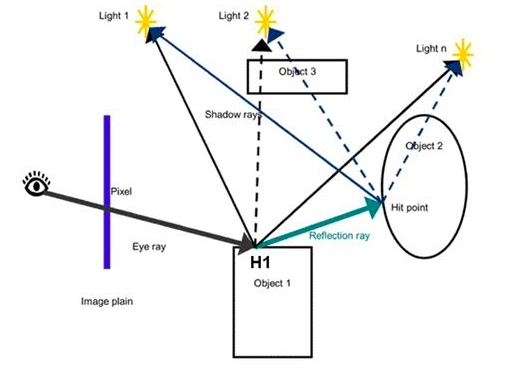
\includegraphics[scale=0.55]{img/trace.png}}
	\caption{Алгоритм обратной трассировки}
	\label{fig:trace}
\end{figure}

Эффективность процедуры определения пересечений луча с поверхностью объекта оказывает самое большое влияние на эффективность всего алгоритма. Чтобы избавиться от ненужного поиска пересечений было придумано искать пересечение луча с объемной оболочкой рассматриваемого объекта. Под оболочкой понимается некоторый простой объект, внутрь которого можно поместить рассматриваемый объект, к примеру параллелепипед или сферу. 

В дальнейшем при рассмотрении пересечения луча и объемной оболочкой рассматриваемого объекта, если такого пересечения нет, то и соответственно пересечения луча и самого рассматриваемого объекта нет, и наоборот, пересечение найдено, то возможно, есть пересечение луча и рассматриваемого объекта. 

Преимущества алгоритма:
\begin{itemize}
	\item возможность использования алгоритма в параллельных вычислительных системах.
\end{itemize}

Недостаттки алгоритма:
\begin{itemize}
	\item требуется большое количество высислений;
	\item производительность алгоритма.
\end{itemize}

\subsection{Алгоритм Робертса}

Работа данного алгоритма проходит в 2 этапа:
\begin{itemize}
	\item определение нелицевых граней для каждого тела отдельно;
	\item определение и удаление невидимых ребер \cite{demin}.
\end{itemize}


Для определения, лежит ли точка в положительном подпространстве, используют проверку знака скалярного произведения $(l, n)$, где $l$ --- вектор, направленный к наблюдателю, фактически определяет точку наблюдения; $n$ --- вектор внешней нормали грани. Если $(l, n) > 0$, т. е. угол между векторами острый, то грань является лицевой. Если $(l, n) < 0$, т. е. угол между векторами тупой, то грань является нелицевой.
В алгоритме Робертса требуется, чтобы все изображаемые тела или объекты были выпуклыми. Невыпуклые тела должны быть разбиты на выпуклые части. В этом алгоритме выпуклое многогранное тело с плоскими гранями должно представиться набором пересекающихся плоскостей. Уравнение произвольной плоскости в трехмерном пространстве имеет вид \ref{varnok1}.

\begin{equation}
	\label{varnok1}
	ax+by+cz+d = 0
\end{equation}

В матричной форме \ref{varnok1} выглядит как \ref{varnok2}.

\begin{equation}
	\label{varnok2}
	[x \: y \: z \: 1][P]^T = 0
\end{equation}

В формуле \ref{varnok2} выражение $[P]^T$ = $[a \; b \; c \; d]$ представляет собой плоскость. Поэтому любое выпуклое твердое тело можно выразить матрицей тела, состоящей из коэффициентов уравнений плоскостей, т. е.

\begin{equation}
	M = \begin{bmatrix}
		a_1 & a_2 & ... & a_n           \\[0.3em]
		b_1 & b_2 & ... & b_n           \\[0.3em]
		c_1 & c_2 & ... & c_n           \\[0.3em]
		d_1 & d_2 & ... & d_n           \\[0.3em]
	\end{bmatrix},
\end{equation}

где каждый столбец содержит коэффициенты одной плоскости.

Любая точка пространства может быть представлена в однородных координатах вектором $[S]~=~[x \; y \; z \; 1]$. Более того, если точка $[S]$ лежит на плоскости, то $[S]*[P]^T$ = 0. Если же $[S]$ не лежит на плоскости, то знак этого скалярного произведения показывает, по какую сторону от плоскости расположена точка. В алгоритме Робертса предполагается, что точки, лежащие внутри тела, дают отрицательное скалярное произведение. 

Преимущества алгоритма:
\begin{itemize}
	\item высокая точность вычислений.
\end{itemize}

Недостатки алгоритма:
\begin{itemize}
	\item рост числа трудоемкости алгоритма, как квадрата числа объектов \cite{demin};
	\item работа только с выпуклыми телами.
\end{itemize}

\subsection{Алгоритм, использующий Z-буфер}

В данном алгоритме рассматриваются два буфера. Буфер кадра используется для запоминания атрибутов (интенсивности) каждого пикселя в пространстве изображения, z-буфер --- это отдельный буфер глубины, используемый для запоминания координаты z или глубины каждого видимого пикселя в пространстве изображения. В процессе работы глубина или значение z каждого нового пикселя, который нужно занести в буфер кадра, сравнивается с глубиной того пикселя, который уже занесен в z-буфер. Если это сравнение показывает, что новый пиксель расположен впереди пикселя, находящегося в буфере кадра, то новый пиксель заносится в этот буфер и, кроме того, производится корректировка z-буфера новым значением z. Если же сравнение дает противоположный результат, то никаких действиq не производится. По сути, алгоритм является поиском по х и у наибольшего значения функции $z(x, y)$ \cite{demin}.

Преимущества алгоритма:
\begin{itemize}
	\item элементы сцены заносятся в буфер кадра в произвольном порядке, поэтому в данном алгоритме не тратится время на выполнение сортировок;
	\item произвольная сложность сцены;
	\item поскольку размеры изображения ограничены размером экрана дисплея, трудоемкость алгоритма зависит линейно от числа рассматриваемых поверхностей.
\end{itemize}

Недостатки алгоритма:
\begin{itemize}
	\item трудоемкость устранения лестничного эффекта;
	\item большой объем требуемой памяти.
\end{itemize}


\section{Анализ методов закрашивания}

Методы закрашивания используются для затенения полигонов (или по-
верхностей, аппроксимированных полигонами) в условиях некоторой сцены, имеющей источники освещения.

Существует несколько основных методов закраски:
\begin{itemize}
	\item простая закраска;
	\item закраска по Гуро, основанная на интерполяции значений интенсивности освещенности поверхности;
	\item закраска по Фонгу, основанная на интерполяции векторов нормалей к граням многогранника.
\end{itemize}

\subsection{Простая закраска}

Одной из самых простых моделей освещения является модель Ламберта. Она учитывает только идеальное диффузное отражение света от тела. Считается, что свет падающий в точку, одинаково рассеивается по всем направлениям полупространства. Таким образом, освещенность в точке определяется только плотностью света в точке поверхности, а она линейно зависит от косинуса угла падения. При этом положение наблюдателя не имеет значение, так как диффузно отраженный свет рассеивается равномерно по всем направлениям.

Простая закраска используется при выполнении трех условий:
\begin{itemize}
	\item предполагается, что источник находится в бесконечности;
	\item предполагается, что наблюдатель находится в бесконечности;
	\item закрашиваемая грань является реально существующей, а не полученной в результате аппроксимации поверхности.
\end{itemize}

Большим недостатком данной модели является то, что все точки грани будут иметь одинаковую интенсивность.

\begin{figure}[ph!]
	\center{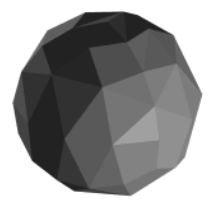
\includegraphics[scale=0.45]{img/draw_simple.png}}
	\caption{Пример простой закраскии}
	\label{fig:draw_simple}
\end{figure}

\subsection{Закраска по Гуро}

Данный алгоритм предполагает следующие шаги:

\begin{itemize}
	\item вычисление векторов нормалей к каждой грани;
	\item вычисление векторов нормали к каждой вершине грани путем усреднения нормалей к граням;
	\item вычисление интенсивности в вершинах грани;
	\item интерполяция интенсивности вдоль ребер грани;
	\item линейная интерполяция интенсивности вдоль сканирующей строки.
\end{itemize}

Достоинства:

\begin{itemize}
	\item хорошо сочетается с диффузным отражением;
	\item изображение получается более реалистичным, чем при простой закраске.
\end{itemize}

Недостатки:

\begin{itemize}
	\item данный метод интерполяции обеспечивает лишь непрерывность значений интенсивности вдоль границ многоугольников, но не обеспечивает непрерывность изменения интенсивности.
\end{itemize}

\begin{figure}[ph!]
	\center{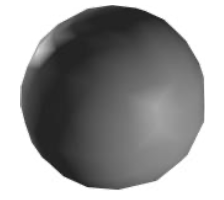
\includegraphics[scale=0.45]{img/draw_guro.png}}
	\caption{Пример закраски по Гуро}
	\label{fig:draw_guro}
\end{figure}

\subsection{Закраска по Фонгу}

При такой закраске, в отличие от метода Гуро, вдоль сканирующей строки интерполируется значение вектора нормали, а не интенсивности. 

Шаги алгоритма:

\begin{itemize}
	\item вычисление векторов нормалей в каждой грани.
	\item вычисление векторов нормали к каждой вершине грани.
	\item интерполяция векторов нормалей вдоль ребер грани.
	\item линейная интерполяция векторов нормалей вдоль сканирующей строки.
	\item вычисление интенсивности в очередной точке сканирующей строки.
\end{itemize}

Достоинства:
\begin{itemize}
	\item можно достичь лучшей локальной аппроксимации кривизны поверхности.
\end{itemize}

Недостатки:
\begin{itemize}
	\item ресурсоемкость;
	\item вычислительная сложность.
\end{itemize}


\begin{figure}[ph!]
	\center{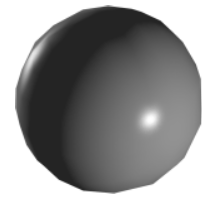
\includegraphics[scale=0.45]{img/draw_phong.png}}
	\caption{Пример закраски по Фонгу}
	\label{fig:draw_phong}
\end{figure}

\section{Алгоритмы моделирования броуновского движения}

Броуновское движение --- беспорядочное движение малых частиц, взвешенных в жидкости или газе, происходящее под действием молекул окружающей среды. 

\begin{figure}[ph!]
	\center{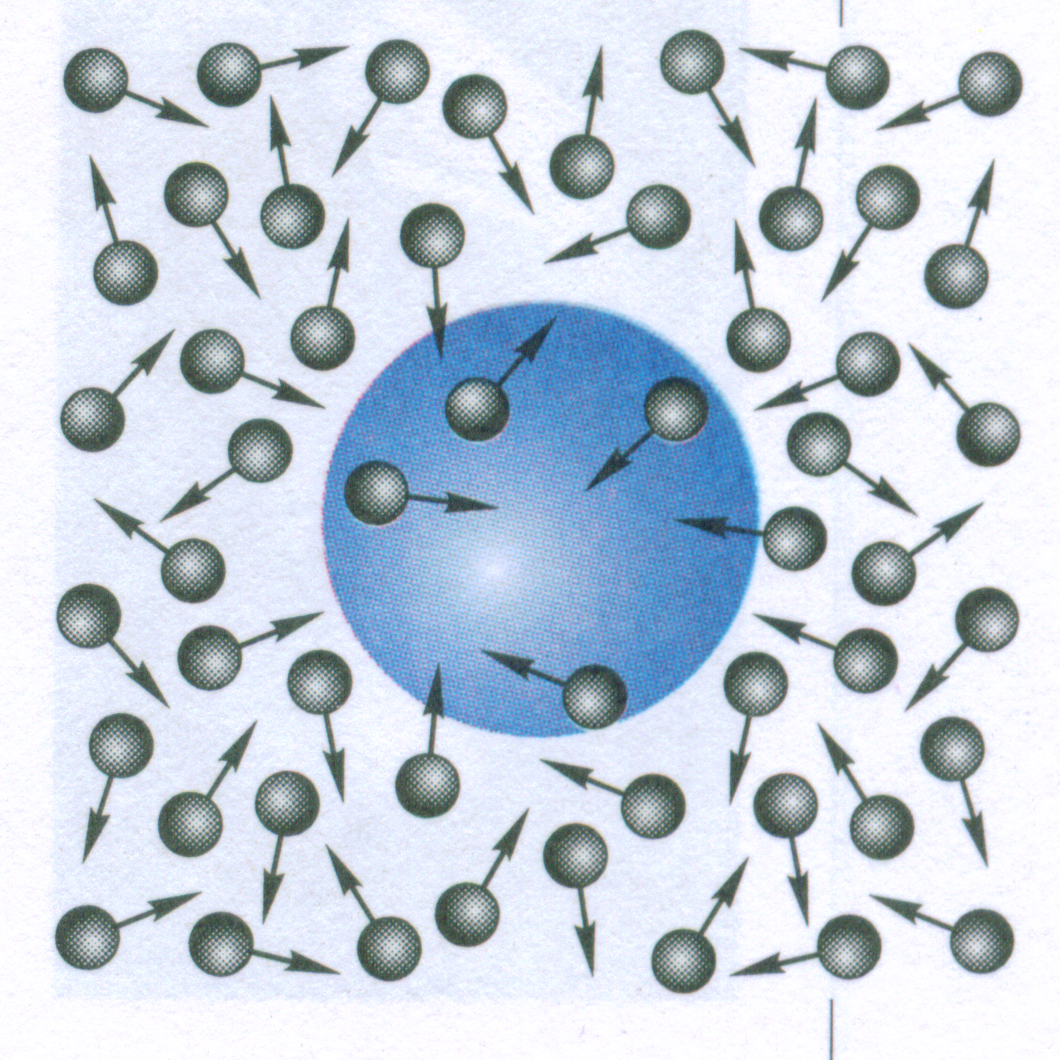
\includegraphics[scale=0.2]{img/brown_movement.png}}
	\caption{Броуновское движение}
	\label{fig:brown_movement}
\end{figure}

Рассмотрим случайный процесс (случайную величину) $X(t)$, заданную на отрезке $[0,T]$.

Случайный процесс  $X(t)$ называется одномерным броуновским движением на интервале $[0,T]$, если он обладает следущими свойствами:
\begin{itemize} 
	\item $X(0) = 0$ почти наверное и $X(t)$ - почти наверное непрерывная функция на $[0,T]$
	\item $X(t)$ - процесс с независимыми приращениями
	\item  $X(t)$ -  процесс с приращениями, распределёнными нормально.
\end{itemize}

Отметим следующие свойства броуновского движения:
\begin{itemize} 
	\item $X(t)$ почти наверное нигде не дифференцируем 
	\item  $X(t)$ - марковский процесс (не обладает памятью), т.е. если известна величина $X(t)$, то при $t_1$ < $t$ < $t_2$ величины $X(t_1)$ и $X(t_2)$ независимы.
	\item Фрактальная размерность графика $X(t)$ равна 1.5
	\item Приращение $X(t)$ обладает свойством статистического самоподобия: для любого $r > 0$
	\begin{equation}
		X(t+ \bigtriangleup t) = \frac{1}{\sqrt{r}}(X(t+r\bigtriangleup t) - X(t))
	\end{equation}
	\item Стационарность приращений: дисперсия приращения зависит только от разности моментов времени
	\begin{equation} \label{1.6}
		D(X(t_2) - X(t_1)) = \sigma^2|t_2-t_1|
	\end{equation}
	\item Математическое ожидание приращения равно
	\begin{equation}
		E(|X(t_2) - X(t_1)|) = \sqrt{\frac{2}{\pi}}\sigma\sqrt{|t_2-t_1|}
	\end{equation}
\end{itemize}

Для моделрования броуновского движения можно воспользоваться разными алгоритмами. Рассмотрим несколько из них.

\subsection{Классическое броуновское движение}

Проще всего реализовать дискретную реализацию броуновского движения, рассмотрев последовательность $x_0$ = 0, $x_{n+1} = x_n + g_n$, где $g_n$ - случайная величина, имеющая нормальное распределение (например, $N(0,1)$).

\begin{algorithmic}[1]
	\State $array[N]$
	\State $array[0]\gets 0$
	\For{i = 1,..., $N$}
	\State $array[i+1]\gets array[i] + randomNormal(0,1)$
	\EndFor
\end{algorithmic}

\subsection{Алгоритм срединных смещений}

Метод случайного срединного смещения основан на работах Н.Виннера , он более сложен, чем метод из предыдущего параграфа, однако используется для конструктивного доказательства существования броуновского движения, а также для построения фрактальной интерполяции (когда необходимо чтобы кривая проходила через заданные точки интерполяции). Метод также может быть обобщен на случай $n$-мерных броуновских движений.

Алгоритм случайного срединного смещения вычисляет значения $X(t)$ в диадических рациональных точках вида $\frac{k}{2^n}$ $\in$ [0,1]. Последовательно вычисляются значения в середине отрезка [0,1], а затем в серединах отрезков [0, $\frac{1}{2}$] и [$\frac{1}{2}, 1$] и т.д. На каждом шаге итерации должен выполнятьяс закон дисперсии для приращения в вычисленных точках. Параметр $\sigma$ определяет масщтаб по вертикальной оси, не влияя на фрактальную размерность графика. 

Вход: $N$, 	$\sigma$ // $N$ - число шагов алгоритма, при этом всего $2^N + 1$ точек интерполяции, $\sigma$ - параметр вертикального масштаба, коэффициент дисперсии

Выход: массив значений $\left\{X(\frac{k}{2^N})\right\}_{k=0}^{2^N}$ // реализация броуновского движения $X(t)$ на дискретном множестве точек вида $t_k = \frac{k}{2^N}$, k $\in$ $[0, 2^N]$

\begin{algorithmic}[1]
	\State $X(0)\gets 0$
	\State $X(1)\gets \sigma g$ // g - случайная величина, распределенная нормально с параметрами $N(0,1)$
	\For{j = 1,..., N}
	\For{i = 1,..., $2^{N-1}$}
	\State $X((2i - 1) 2^{N - j})$$\gets$ $X((i - 1)2^{N-j+1}) + X(i2^{N - j + 1}) + \frac{1}{2^{(j+1)/2}}$$\sigma$ g
	\EndFor
	\EndFor
\end{algorithmic}

\subsection{Фрактальное броуновское движение}

Фрактальное броуновское движение (ФБД) уже не является марковским процессом, а обладает некорой "памятью". Кроме того, вводя параметр $0 < H < 1$ можно получитьодномерное ФБД размерности $d = 2 - H$ и двумерное ФБД размерности $d = 3 - H$ .
Заметим, что классическое броуновское движение получается как частный случай при $H = 0.5$. Для апроксимации ФБД нет простого метода, вроде суммирования нормальных случайных величин, как в случае классического броуновского движения. Для апроксимации ФБД наиболее удобно использовать преобразования Фурье.

Рассмотрим случайный процесс (случайную величину) $X(t)$, заданную на отрезке $[0, T]$.

\textit{Случайный процесс}  $X(t)$ называется одномерным фрактальным броуновским движением на интервале $[0, T]$, если он обладает следущими свойствами:

\begin{itemize}
	\item $X(0) = 0$ почти наверное и $X(t)$ - почти наверне непрерывная функция на $[0, T]$
	\item  $X(t)$ - процесс с приращениями, распределенными нормально
\end{itemize}

Отметим следующие свойства фрактального броуновского движения:

\begin{itemize}
	\item $X(t)$ почти наверное нигде не дифференцируем 
	\item Фрактальная размерность графика $X(t)$ равна $2 - H$
	\item Процесс $x(t)$ не обладает свойством независимости приращений
	\item Приращение \textit{X(t)} обладает свойством статистического самоподобия: для любого $r$ > 0
	\begin{equation}
		X(t+ \bigtriangleup t) = \frac{1}{\sqrt{r}}(X(t+r\bigtriangleup t) - X(t))
	\end{equation}
	\item Стационарность приращений: дисперсия приращения зависит только от разности моментов времени
	\begin{equation} \label{1.6}
		D(X(t_2) - X(t_1)) = \sigma^2|t_2-t_1|^{2H}
	\end{equation}
	\item Математическое ожидание приращения равно
	\begin{equation}
		E(|X(t_2) - X(t_1)|) = \sqrt{\frac{2}{\pi}}\sigma|t_2-t_1|^H
	\end{equation}
\end{itemize}

\newtheorem{theorem1}{Теорема}
\begin{theorem1}
	Если $X(t)$ - ФБД с параметром $H$, то его спектральная плотность 
	\begin{equation}
		S(f) \propto \frac{1}{f^{2H+1}}
	\end{equation}
\end{theorem1}

Идея метода состоит в следующем. Строится преобразование Фурье для искомого ФБД в частной области, задавая случайные фазы и подбирая амплитуды, удовлетворяющие свойству из Теоремы 1. Затем получаем ФБД во временной области с помощью обратного преобразования Фурье.

Будем моделировать дискретный аналог ФБД, то есть наша цель- получить величины $\left\{X_n\right\}_{n=0}^{N-1}$, апроксимирующиеФБД в точках $n$. Воспользуемся формулой дискретного преобразования Фурье

\begin{equation}
	\hat{X_n} = \sum_{k=0}^{N-1}X_ke^{-2\pi kn/N}
\end{equation}

и обратного дискретного преобразования Фурье

\begin{equation}
	X_n = \sum_{k=0}^{N-1}\hat{X_k}e^{2\pi kn/N}
\end{equation}

Далее будем рассматривать только четные значения $N$, а для применения метода \textit{быстрого дискретного преобразования Фурье} нужно, чтобы $N=2^M$, $M \in \mathbb{N}$. Метод быстрого дискретного преобразования Фурье  реализован во многих системах компьютерной алгебры. Он позволяет сократить вычисления в $\frac{2N}{\log_2N}$ раз.

Для того, чтобы получающиеся величины $X_n$ были вещественными мы наложим условие сопряженной симметрии:

\begin{equation}
	\hat{X}_0, \hat{X}_{N/2} \in \mathbb{R}, \hat{X}_n = \hat{X}_{N-n}, n = 1,...,N/2-1
\end{equation}

Фильтрация относится к той части моделирования, когда мы заставляем коэффициенты преобразования Фурье удовлетворять степенному закону из Теоремы 1:

\begin{equation}
	|\hat{X}_n|^2 \propto \frac{1}{n^{2H+1}}, n = 1,...,N/2
\end{equation}

Для этого возьмем

\begin{equation}
	\hat{X}_n = \frac{ge^{2\pi iu}}{n^{H+0.5}}
\end{equation}

где $g$ - независимые значения нормально распределенной случайной величины с параметрами $N(0,1)$, а $u$ - независимые значения равномерно распределенной на отрезке [0,1] случайной величины. Оставшиеся коэффициенты вечислим из сотношений 1.15.

Для вычисления искомой аппроксимации ФБД $\left\{X_n\right\}_{n=0}^{N-1}$ применим обратное дискретное преобразование Фурье к набору $\left\{\hat{X}_n\right\}_{n=0}^{N-1}$.

Вход: $H \in (0,1)$, $N=2^M$, $M \in \mathbb{N}$ // $H$ - параметр ФБД, размерность графика равна $d = 2 - H$, $N$ - параметр, определяющий количество точек дискретизации ФБД.

Выход: массив значений $\left\{X_n\right\}_{n=0}^{N-1}$ // дискретная апроксимация ФБД в последовательные моменты времени n.

\begin{algorithmic}[1]
	\State $\hat{X}_0\gets g$
	\For{j = 1,..., N/2-1}
	\State $\hat{X}_j \gets \frac{ge^{2\pi iu}}{j^{H+0.5}}$
	\EndFor
	\State $\hat{X}_{N/2} \gets \frac{g\cos(2\pi iu)}{(N/2)^{H+0.5}}$ // Здесь $\cos$ — вещественная часть комплексной экспоненты $e$
	\For{j = N/2+1,..., N-1}
	\State $\hat{X}_j \gets \overline{\hat{X}_{N-j}}$
	\EndFor
	\State $X \gets convert(\hat{X})$ // Вектор $X = \left\{X_0,...,X_{N-1}\right\}$ получается обратным дискретным преобразованием Фурье из вектора $\hat{X} = \left\{\hat{X}_0,...,\hat{X}_{N-1}\right\}$.
\end{algorithmic}

\section*{Вывод}
В данном разделе было представлено описание объектов сцены, а также обоснован выбор алгоритмов, которые будут использованы для ее визуализации.

Для удаления невидимых линий и поверхностей выбран алгоритм Z-буфера, так как он обладает важными преимуществами --- высокой скоростью работы и возможностью отображать сцены произвольной сложности.
Также была выбрана локальная модель освещения Ламберта, так как программа не должна выводить реалистичного изображения и должна иметь наиболее высокую производительность, и закраска по Гуро, так как алгоритм достаточно быстр, и он хорошо сочетается с выбранным ранее Z-буфером.

Для моделирования броуновского движеняи был выбран алгоритм срединных смещений, так как он позволяет наиболее реалистично изобразить броуновское движение, а также легко обобщается для случая $n$-мерных движений. Также данный алгоритм содержит меньшее количество вычислений чем алгоритм Фурье-фильтрации, то есть вычсленяи будут выполняться быстрее. 
